\section{Problem (2)}

	A $2.5 \ kg$ toy car can move along an $x$ axis; the figure gives $F_{x}$ of the force acting on the car, which begins at rest at time $t = 0$. The scale on the $F_{x}$ axis is such that the point $F_{xs} = 20.0 \ N$.

	\begin{figure}[H]
		\begin{center}
			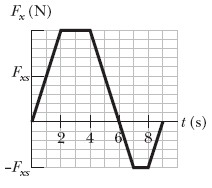
\includegraphics[scale=1]{hw9_problem2}
			\caption{Illustration of Problem 2}
			\label{fig:hw9_problem2}
		\end{center}
	\end{figure}

	\subsection{Question (a)}

		What is $p$ at $t = 1.0 \ s$?

		\textbf{R:}

		\begin{align}
			p_{i} = \ &(2.5 \ kg)(0 \ m/s) = 0& \notag \\
			p_{f} = \ &I = F_{ave}\Delta t& \notag \\
			p_{1.0 \ s} = \ &\left(\frac{F_{xs}}{2}\right)(1 \ s)& \notag \\
			 = \ &10.0 \ N \times s&
		\end{align}

	\subsection{Question (b)}

		What is $p$ at $t = 2.0 \ s$?

		\textbf{R:}

		\begin{align}
			p_{2.0 \ s} = \ &\left(\frac{F_{xs} + 2F_{xs}}{3}\right)(2 \ s)& \notag \\
			= \ &(20.0 \ N)(2 \ s)& \notag \\
			= \ &40.0 \ N \times s&
		\end{align}

	\subsection{Question (c)}

		What is $v$ at $t = 5.0 \ s$?

		\textbf{R:}

		\begin{align}
			p_{5.0 \ s} = \ &\left(\frac{F_{xs} + 2F_{xs} + 2F_{xs} + 2F_{xs} + F_{xs}}{6}\right)(5 \ s)& \notag \\
			= \ &(26.\bar{6} \ N)(5 \ s)& \notag \\
			= \ &133.\bar{3} \ N \times s& \notag \\
			v_{5.0 \ s} = \ &\frac{p_{5.0 \ s}}{m}& \notag \\
			= \ &\frac{133.\bar{3} \ N \times s}{2.5 \ kg}& \notag \\
			= \ &53.\bar{3} \ m/s&
		\end{align}
